\documentclass[conference]{IEEEtran}

% import custom packages
\usepackage{amsmath,amssymb}
\usepackage{graphicx}
\usepackage{hyperref}
\usepackage{cleveref}

\newcommand{\projectname}{NFC WorkTracker}
\newcommand{\surveyquestion}[3]{%
	\noindent\textbf{#1}
	
	\noindent User A: \textit{#2}\\
	User B: \textit{#3}
}

\graphicspath{{images}}

\title{\projectname\\\Large{A novel approach to put-your-phone-down applications.}}
\author{Torge Rosendahl}

\begin{document}
\maketitle

\begin{abstract}
foo bar
\\
This report was written as part of the McGill ECSE 542 --- Human-Computer Interaction course.
\end{abstract}

\begin{IEEEkeywords}
foo bar, foo, bar
\end{IEEEkeywords}

\section{Motivation}
For me as a person it has always been difficult to ``just put my phone down'' when I have to get stuff done. And that has not become easier with more social media platforms. It is a known problem, than especially Generation Z has trouble focusing on work [SOURCE], due to being used to regularly looking at their phone. More and more young people have difficulties to put their phone away from time to time. What often helped me in such a situation was to put my phone away, ideally in another room, to just not think about having to reach it. But especially the part of putting your phone in another room is often something that is easier said than done. Especially for students that have to study on their own, often at home, this can make the everyday life much more difficult.

Over the last years, many apps have arisen that offer motivation to not use your phone. This is done either through a (soft) lockdown of the device, like with the \textit{OnePlus ZenMode}\footnote{\url{https://www.oneplus.com/global/blog/product/zen-mode-explained}} or Android's \textit{Focus Mode}\footnote{\url{https://blog.google/products/android/android-focus-mode/}}, or through some kind of gamification\footnote{In the example of \textit{Forest}, this includes planting virtual and real trees. Other apps, for example, let you compare yourself with friends.}, for example in \textit{Forest}\footnote{\url{https://www.forestapp.cc/}}. An additional feature most of these apps have is the recording of hours where the app was active.

For some people, these apps are able to provide a routine of starting their ``session'' in the app, then working on whatever they have to work on and finally stopping tracking in the app. For other people, however, it is difficult to develop this routine, because just looking at your phone before starting work might drag them into a notification or some social media app, effectively stopping them from starting to work rather than motivating them. Additionally, they might be waiting for a phone call or want to be able to get some specific kind of notifications. Traditional time-tracking-apps, however, often mute your device, or even completely lock it down for a user-defined period of time to prevent ``accidental'' usage.

The act of putting the physical object [phone] down, however, can be much easier correlated with a productive time in the brain[SOURCE? or delete]. It also allows you to hear that important phone call you do not want to miss ring through your apartment.

The {\projectname} combines the act of putting down your phone when you start working with the additional functionality of an app. This app will track the time, for which your phone did stay in touch with the surface you put it on. Having an app track you not only gives you an additional pinch of motivation to not touch your phone mid-work, it also allows additional features, like an automated recording of worked hours.

\section{Application Concept}
As the reader might have guessed by this point, the technology used for checking the presence of a \textit{surface} that the phone is laid upon is Near Field Communication (NFC). This requires a secondary device that acts as the surface, in this case provided by a passive NFC tag. Such tags come in the form of actual key tags, plastic cards or as simple stickers. For a general purpose application, stickers are the best choice. The sticker can be placed on the surface where the user wants to have their phone when working.

\subsection{NFC Usage \& Specification}
\label{sec:nfc-details}
NFC has a maximum communication range of 20 cm \cite{nfcsurvey}, which allows for sufficiently easy placement of the phone but guarantees connection loss when the phone is moved. NFC tags can hold any binary data, often stored on the tag as NDEF\footnote{NFC Data Exchange Format} messages which can hold multiple records. These record can hold a multitude of different things, in my case there will be single message with one record that holds an application-defined MIME-type\footnote{Multipurpose Internet Mail Extensions (MIME) is used to specify the data format of a chunk of data, for example \textit{text/html} for websites.} where the content is an ID the identifies the tag\footnote{Actually, the ID is currently neither unique, nor used. The app currently relies on the existence of this data record, which is enough to fulfill the specified use cases.}. The data specified on a \projectname{} tag uses the type \textit{application/ca.mcgill.nfcworktracker.tag}, which contains the package name of the project and is therefore application-specific. The following data is the tag's ID,. represented as plain text.
%TODO before submit: check formatting of mime type -> force into one line

\subsection{Application Features}
The usage of the app itself is very intuitive. Just telling the user (through means that remain to be defined for now) that they can put their phone down onto an NFC tag to track their work hours gives them all the information they need to actively use the system. The NFC tag itself is thereby a valid signifier for where to place the phone, and most young people nowadays have used NFC before, for example for card-less payment.

The important part this app needs to cover as well to become intuitively usable by everyone is providing the user with all essential information, as well as guiding them through the setup process. This setup process consists of buying an NFC tag (or multiple), choosing a place to put it for daily work and then registering it to work with the app.
%guiding through buying an NFC "tag" (generally meaning sticker, card, or other)
The user will, for the submitted project state, not be guided through the process of picking and purchasing an NFC tag, because any NFC tag works, as long as it is writable. NFC tags come in different shapes and sizes, most often they are found as stickers or in a credit card format. The remaining part of the setup and usage process is guided by the app itself.

The setup process is by far less intuitive than the usage process, so I expected from the beginning that the setup process has the most potential for improvement.

\section{First Mockup}
\subsection{Implementation Details and Process}
This section will explain the first implementation of the \projectname{}, which is intended to be a proof-of-concept and to be used for the feedback round. This first version of \projectname{} already supports all the required features. This includes tracking of work hours, setting up the application and corresponding NFC tags and viewing the tracking history. I will present these features in the order I implemented them in. This allows me to give some insight into my implementation process along with the presentation of the results.

\subsubsection{Home Screen}
The home screen is the landing page when the user starts the app. It has buttons to setup/create a new tag and to show the tracking history.

\subsubsection{Active Tracking}
The app has to support tracking the presence of an NFC tag in the background. While the user is of course not intended to use their phone during tracking, there is no way to prevent them from for example looking at a notification of setting up some other work-related things on their phone, like turning on Do Not Disturb. Therefore, within the environment of Android, the tracking is implemented as a service. Android differentiates between background and foreground services. The former are used for processing details in the background, but are not allowed to access interactive resources [SOURCE]. Therefore, \projectname{} uses a foreground services. This, additionally to being able to access the NFC hardware, also allows the app to show a notification to the user confirming that tracking has successfully been started. This kind of confirmation is really helpful to build trust into the tracking functionality.

Throughout the implementation, I stumbled upon a minor inconvenience: Android only allows NFC tags to open activities. An activity is something that is displayed to the user, like the main screen of basically any app. Therefore, we cannot start our tracking service directly from a tag. The workaround to overcome this solution is to ??? [CHECK]!!!!!!! might be that the constraint rather was that startForeground in the service only works from activities!

%TODO fix previous
%TODO ref show screenshot of notificatin in text
%TODO write about exact flow of put down -> notificatino -> until stop

\begin{figure}
	\centering
%	\includegraphics[width=\linewidth]{}
	\caption{Screenshot of the ``tracking active''-notification. It is shown whenever the tracking service is currently running.}
	\label{fig:notification}
\end{figure}

When the user stops the tracking while the phone is still on the tag, the tag will from then on be ignored. The user has to lift the phone off the tag and put it back down to re-start the tracking.

\subsubsection{History View}
The next section I implemented was the history view. Through this, the user can see the past usage of the tracking functionality.

The history itself is stored in an SQLite database within the application, using Android's Room abstraction layer[SOURCE]. This allows persistent storage between sessions and offers an intuitive way for the developer to access structured data through SQL queries.

The home screen of \projectname{} has a button that launches an activity to display the history. This history-activity acts independently from the rest of the app. For example, showing the history does not interfere with a possible active work tracking process. The history view lists all past history entries. In the current (first) implementation, each entry is represented by it's start and end time which is displayed as a date/time combination in the user interface. Displayed times and dates are localized and work across different time zones. However, for privacy reasons, the timezone is not stored with the history entry, so if you move to a different time zone, the times in your history will appear shifted to your \textbf{new} time zone. From a design perspective, the app would even work if you were to move timezones during tracking.

In the application bar (the top bar with the back arrow), there is a three dot-menu that has a ``clear history'' entry.

\subsubsection{Setup Process}
When the base construct of the app was functional, I went on to do the setup process. This process is, like the history, started as a new activity on the press of a button on the home screen of the app.

First, I drew some sketches on what I want the setup process to look like. It is a step-by-step instructions, so a series of consecutive screen makes sense. Only when the current step has been completed, either by the app or by the user, the setup process will display instructions for the next.
%TODO show and explain sketches!
%TODO explain all the fragments and their job.
The introduction fragment (FIGREF) is there to prepare the phone for the upcoming setup process. It makes sure that the user has NFC turned on and instructs them on how to place the to-be-written NFC tag. The ``setup'' fragment instructs the user to place the phone on the tag in question (FIGREF) and then waits for that to happen. Then, the tag is written and the user is informed on the outcome, either success (FIGREF) or failure (FIGREF).

Second, I implemented the sketches into Android layout files and added the logic flow. Every screen from the sketches is represented by it's own fragment, which represent replaceable sub-layouts in Android activities. For activities that display fragments, Android allows the specification of a navigation graph, to change fragments in a structured manner. A simplified version of that navigation graph is shown in \cref{fig:nav-graph}. At this point in the implementation, I added temporary buttons to all the fragments that allow me to navigate along the defined actions, to be able to pretend all the read- and write-interaction with the tag.

\begin{figure}
	\centering
	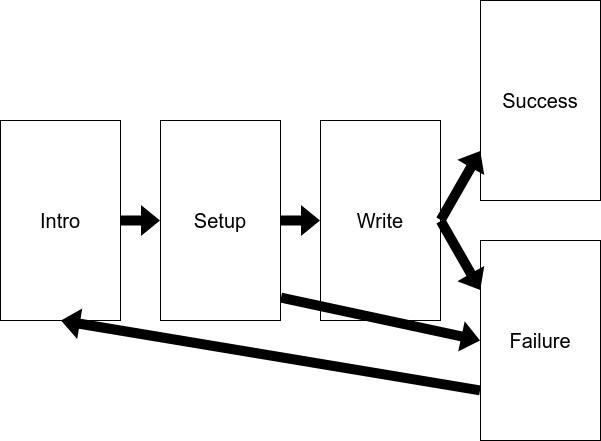
\includegraphics[width=\linewidth]{nav-graph.drawio.png}
	\caption{Simplified version the setup-activity fragment navigation graph.}
	\label{fig:nav-graph}
\end{figure}

Finally, I added all the functionality to the fragments. The fragments most importantly display setup instructions, but some of them have additional logic for interaction with the tag. The intro fragment just statically displays the preparation instructions. The second fragment instructs the user to put their phone down onto an NFC tag. This fragment can only advance to the following step if a tag is detected. Therefore, as soon as it is created, it starts actively looking for tags. For this to work, the automatic (system-wide) NFC detection is disabled in this step. Automatic NFC detection will be re-enabled as soon as the setup activity closes (with or without a successful tag write). When this second setup step finds an NFC tag nearby, it automatically advances to the write step. This fragment, when it is started, will attempt to write a new NDEF message to the tag, containing a record as defined in \cref{sec:nfc-details}. Since the write process finishes almost instantaneously, this fragment does in reality not show. However, in case the write process does take longer for whatever reason, it still displays a ``write in progress''-screen. When the write is completed, the app displays a screen that confirms this success to the user and gives a suggestion on how to proceed. In case the write fails, a failure screen is displayed, with the option to either try again now or quit the setup activity.

\subsection{Runtime Requirements}
To use the app, a small amount of things are required:

\begin{itemize}
	\item Android phone, with minimum Version 8.0 (Oreo)\\
	and has NFC-capable hardware.
	\item NFC tag, that is capable of communicating with phone\\
	(correct NFC technology)\\
	and is writable.
\end{itemize}

\section{Feedback Round}
%user A: JAM, user B: VF
To get an insight into what users think off this first state of the app, I sent out a first copy of the app to two friends. Both testers are students, which matches the discussed target user group.
%TODO can I put some info about the two's details?
Both users were instructed to run through the setup process and use the app as far as possible. I created a test instruction document to get comparable results. This document also included a short survey at the end. The following section discusses the results that came up throughout testing.

One thing that came up pretty quickly during testing is that NFC apparently is handled very differently across different android versions and OEMs. While on my testing device everything seemed to work, both users reported different issues with regard to the tracking. For user A, the tracking stopped every time the screen turned off. This is probably related to power saving measures taken by the phone's manufacturer. The other user reported that the tracking did not stop when the phone was lifted. In return, the tracking also did not stop when the was locked. Within the limited time of this project scope, I was unable to come up with a fix for that. There is however a potential solution that will be discussed later. For the sake of this report, I told both user to pretend the app works. User A disabled the automatic screen timeout for the time testing and user B was instructed to stop the tracking manually, through the button on the notification (see \cref{fig:notification}).

\subsection{Post-Test Survey}


\section{Design Iteration}
%iteration implementation
%changes made to adapt to what the user requested/requires/had struggles with
%foremost: correlation between feedback and changes!
%TODO this is just a test study
%TODO app has to be brought into pulishable state
%TODO then a bigger study can analyze actual usage and usefulness
%TODO I would like to a comparative study of with vs without
%TODO Then, based on that, new cimplementations can be made

\section{Conclusion}
%basic important task: evaluate personal findings with this

\subsection{Final Feedback}
%get feedback for "final" design. reflect on that.
%I give the imporved/working version with their feedback implemented and get their reacction.
%Either: It is not perfectly usable. Or: There is more critique. Changes they did not know they need, or changes they requested but dont like now.

\subsection{Future Perspective}
I will transfer this project into the hands of \textit{vastivety}\footnote{\textit{vastivety} is an organizational level under which a friend and I work on open source projects in our free time. \url{https://vastivety.github.io}.} and keep on developing it with a friend of mine. I think this app has potential to be used by a broader range of people, and I will use this platform to push towards bringing {\projectname} into the known Android app stores.

\section*{Acknowledgement}
I would like to thank my testers that really supported the development process. Without your constructive feedback this project would not be where it is right now. I would also like to thank Professor Cooperstock for his input into the selection of this project, as well as pointing me in the right direction when it came to this report.

%Note bib style from IEEE, see
% https://ieee-dataport.org/sites/default/files/analysis/27/IEEE%20Citation%20Guidelines.pdf

\bibliographystyle{IEEEtran}
\bibliography{IEEEabrv,sources}

\appendices
\section{Post-Test Questionnaire Answers}
\label{app:questionnaire}
The following is a close-to-original version of the post test questionnaire. I removed a few questions that gave no additional insight and edited the other questions to give some context with regard to the removed parts. Grammatical or spelling errors in users' answers have been copied from their questionnaire.

\surveyquestion{Did you trust the app in setting up everything correctly?}{
	Yes.
}{
	I think that overall, the set up went fine. However, I have the impression that my smartphone usage is being observed because of the word “tracking”. I do not want the app developer to know what I do on my phone. I know that it is only measuring the time when on the tag but overall I was struggling with its trustworthiness.
}

\surveyquestion{What step did you struggle most with?}{
	Finding a writable tag that I can use.
}{
	Understanding whether everything worked or not. The notification that the tracking is active did not stop when taking away the phone from the tag so I am not sure whether the app fulfills its purpose yet. I have to end the session by clicking the button in the notification. This needs to be fixed.
}

\surveyquestion{Do you feel like you would have been able to set up the app without this instruction document?}{
	I think I would have been able to do that. It's pretty self-explanatory.
}{
	Yes, the app is self-explanatory. However, there could be a menu in the app with the steps and suggested using practices so everybody can make the most out of their experience with the app.
}

\surveyquestion{How do you think about different session types? Imagine taking notes and setting a color for a specific session through the history menu; or using multiple hardware tags for different type of work.}{
	Good idea. It could also be useful to take notes for the current session on the home screen of the app. Having tags for different work is a good idea. It could also be useful to be able to filter the history for those different activity types and display summed up time for those activities per week/month.
}{
	Okay, but having a pop-up where I can directly set a text-tag for the period at hand would be better. I love the idea of different tags.
}

\surveyquestion{What other features do you miss?}{
	Being able to track while the app is in the background/closed. Deleting single items from the tracking history.
}{
	It can be useful to have the feature that makes it possible starting multiple sessions at once. It would also be nice to include a feature that automatically lock the phone when on the tag and not unlocking it before the next interaction with a tag. It would be nice if the session will also be shown in the app (such as “active”) and if the session history updates automatically when ending a session.
}

\surveyquestion{Do you have anything else to say?}{
	The app's color scheme is a bit off (status bar colors, see screenshot).
}{
	--
}

\end{document}

